%<dscrpt>Exercice de géométrie avec des complexes.</dscrpt>

\begin{figure}[!ht]
 \centering
 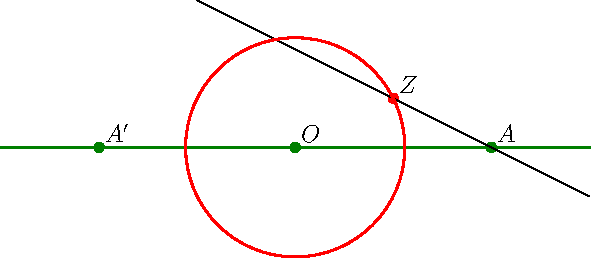
\includegraphics{Ecomp8_1.pdf}
 \caption{Points $A$, $A'$, $Z$}
 \label{fig:Ecomp8_1}
\end{figure}
Soit $a$ un nombre réel strictement positif. Dans un plan muni d'un répère orthonormé d'origine notée $O$, on considère les points $A$ (d'affixe $a$) et $A'$ (d'affixe $-a$).\newline
Pour tout nombre complexe $z\neq a$, on pose
\begin{displaymath}
 m = \overline{z}\,\frac{z-a}{\overline{z}-a}
\end{displaymath}
et à tout point $Z$ d'affixe $z$, on associe le point $M$ d'affixe $m$.
\begin{enumerate}
 \item Montrer que $Z$ et $M$ sont sur un même cercle de centre $O$.
 \item Soit $\alpha$ un argument de $z-a$ et $\theta$ un argument de $z$. Préciser un argument $\mu$ de $m$ en fonction de $\theta$ et $\alpha$ puis en déduire que la droite $(AZ)$ est parallèle à la bissectrice de $(\overrightarrow{OZ},\overrightarrow{OM})$.
 \item Montrer que
\begin{displaymath}
 \forall z\not\in \R :\hspace{0.5cm} \frac{m-z}{z-a} = i\,\frac{2a\Im z}{|z-a|^2},\hspace{1cm}\frac{m+a}{m-z} = i\,\frac{a^2-|z|^2}{2a\Im z}
\end{displaymath}
Que peut-on en déduire pour les droites $(ZM)$, $(AZ)$ et $(A'M)$?\newline
Expliquer comment on peut construire géométriquement $M$ à partir de la donnée de $A$ et $Z$.
\end{enumerate}


